\section{Dataset}

\subsection{Core HCI Venues}
% 
To calculate HCI's \xin, we first need to define what is considered an HCI paper so that we can know which are HCI \vs non-HCI citations.
To the best of our knowledge, there is no existing `catalog' of all HCI venues that publish HCI papers.
Thus we refer to two sources to compile a list of core HCI venues: the SIGCHI-(co)sponsored conferences \cite{Upcoming19:online} and Google Scholar's top publications under the ``Engineering \& Computer Science - Human Computer Interaction'' category \cite{HumanCom38:online}.
In addition, we manually added a few venues we consider should be equivalent to those already in the list, \eg GI, INTERACT, ISWC, OzCHI, and NordiCHI.

Table \ref{tb:venues} shows the compiled core HCI venues
% \footnote{Some venues changed their name at some point, thus we at times included multiple identifiers for the same venue.}. 
For each venue, we manually extract a subset of words from its official name to serve as a unique identifier, which we later use in keyword-matching to determine whether a citation is HCI or not.

Admittedly, what is not in this list is not necessarily ``non-HCI''; it is just not included by the two sources we chose.
Nonetheless, we argue that this list approximates the ``boundary'' between HCI and the non-HCI world.
The more we see citations of an HCI paper coming outside of this list (\ie higher \xin), the more likely this HCI paper is having an impact across this ``boundary''.
We hereafter refer to papers published outside of this list as {\bf non-HCI papers}.

\begin{table}
    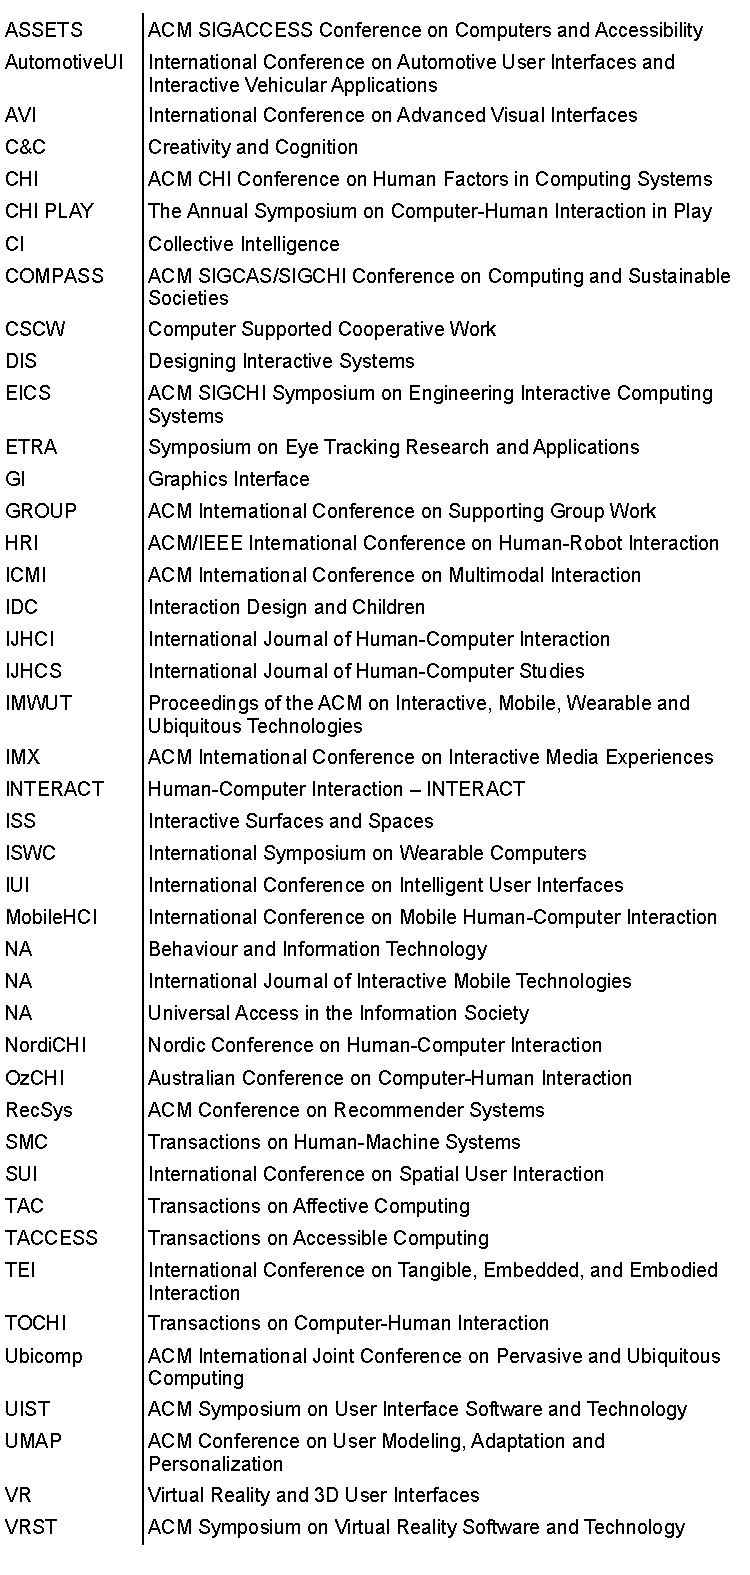
\includegraphics[width=\columnwidth]{figures/hci_venues.pdf}
    \caption{A list of core HCI venues.}
    \label{tb:venues}
\end{table}

\subsection{Citations of CHI, UIST, and CSCW Papers}
% 
Next, we collected DOI data of CHI, UIST and CSCW papers between 2010 to 2020\footnote{Except for CSCW 2020 papers, which the website did not provide.} from the ``What The HCI'' \cite{WhatTheH50:online} website maintained by Kashyap Todi.
We chose CHI, UIST and CSCW because they are three of the most well-recognized HCI venues.
% ---we hereafter refer to papers published in these three venues as {\bf HCI papers}.
% \footnote{Another reason for selecting these three venues is due to convenience because their data was readily available from \cite{WhatTheH50:online}.}.
It is certainly possible to acquire DOI data of other HCI venues (\eg TOCHI) from other sources (\eg ACM Digital Library).


Then, we port the DOI data into the Citation Chaser app \cite{citation47:online} developed by Neal Haddaway, which uses the Lens.org API \cite{TheLensF23:online} to retrieve citations of a paper based on its DOI.
All the citation data was in the \texttt{.ris} format and collected in January 2023.
We did find that this API did not seem to find all the citations. 
% ---the total count was smaller than Google Scholar's.
Thus it is best thought of as a sampling, rather than an exhaustive retrieval, of papers' citations. 
We do not believe such a limitation invalidates the subsequent \xin calculation unless the missing citations were biased (\eg missing citations mostly came from HCI venues only).

% (forward) citations
% bib